\chapter{Experiments}

%\Todo{move to results? or at end of method}
\section{Performance comparison}
Before we go further and present the methods and results of the experiments
it is necessary to introduce some additional terms. Such as metrics to measure
their performance.

\paragraph{Mean squared error (MSE)} is an error measurement that
describes the error/noise between an given or measured reference signal $x$
and  and the reconstruction(noisy approximation) $\tilde{x}$ of it.
Mathematically it is defined as the average of the squared error between two
signals.
%The mean squared error is defined as:
\begin{align}
 MSE = \frac{1}{n} \sum_{i=0}^{n} \left( {\lVert x_i -
\tilde{x}_i\rVert^{2}}\right)
\end{align}
We primarily use it for testing dictionary learning convergence and as a
sub term for the measurement described in the next paragraph.

\paragraph{Peak signal-to-noise ration (PSNR)} describes the ratio between the
error/noise affecting a signal/reconstruction and the maximum possible signal
amplitude. It is expressed in a logarithmic decibel scale.
\begin{align}
 PSNR = 20 \cdot \log_{10} \left(\frac{MAX}{\sqrt{MSE}}\right)
\end{align}
Where $MAX$ is the maximum possible value of our signal. For an 8-bit
image it would be 255. For a 32-bit normalized image it would be 1. And $MSE$ is
the mean squared error between a reference signal and its reconstruction. The
PSNR is undefined for zero noise.

The PSNR is primarily used for comparison of the reconstruction quality of
lossy compression algorithms. Typical values for a lossy reconstruction lie in
a range between 30dB and
50dB.\footnote{\url{http://en.wikipedia.org/wiki/Peak_signal-to-noise_ratio}}
%e.g. relevant for de-noise

\paragraph{Bits per pixel (bpp)} 
For the comparison of compression ratio of images another well known practice is
to measure the required \emph{bits per pixel} short bpp. The bbp are calculated
by dividing the raw image data by the image's dimensions. For example an
uncompressed RGB color image with 8-bit of color depth requires 24-bits per
pixel, respectively a gray scale image with 8-bit for a single channel requires
8-bits. While compression algorithms are able to encode multiple pixels with few
coefficient leading to much lower bpp rates.
Looking at other well known compression algorithms such as JPEG or
JPEG 2000 a common ratio is about $\sim1.8$ bits-per-pixel for average
quality compression( JPEG quality of 50) of an natural image. 
\Todo{example image?, lower bit rates, Lewicki estimate for sparse coding}

Besides the raw pixel data, images formats usually contain a certain amount
of extra data from file headers and meta data. Fortunately we can ignore this
for simplification as it is only a few bytes and not being actual pixel data.

\paragraph{Test data}
In addition to the introduced metrics it is common practice to use some image
sets to compare test results of the different algorithms and parameter
configurations. As the dictionaries are specificaly trained for
reconstruction of the data in the training sets it is mandatory to also use
these image to test the reconstruction and compression quality.
\begin{figure}[h]
\centering
\subfloat{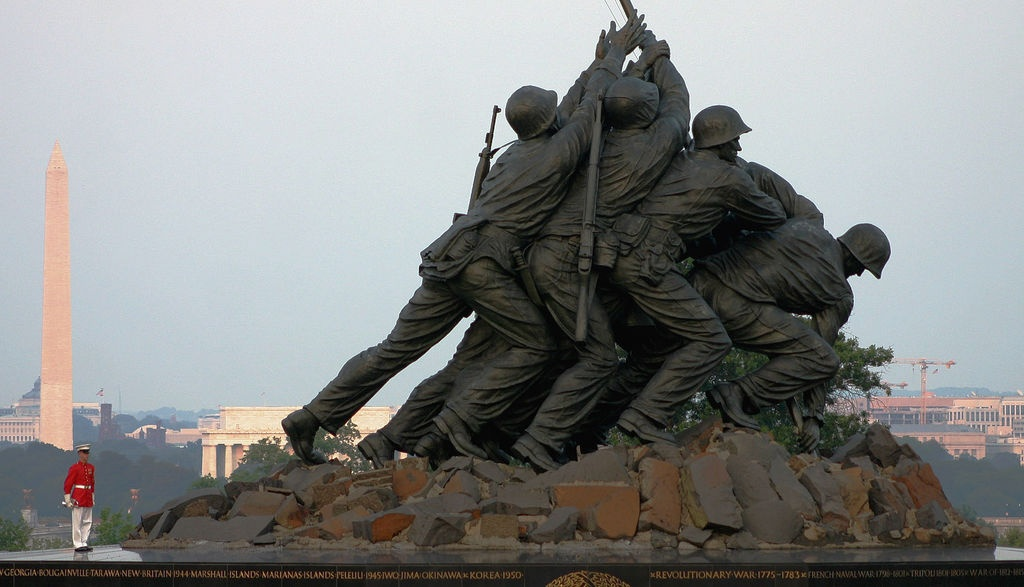
\includegraphics[width = 0.3\textwidth]{images/28979823.jpg}}
\hspace{5mm}
\subfloat{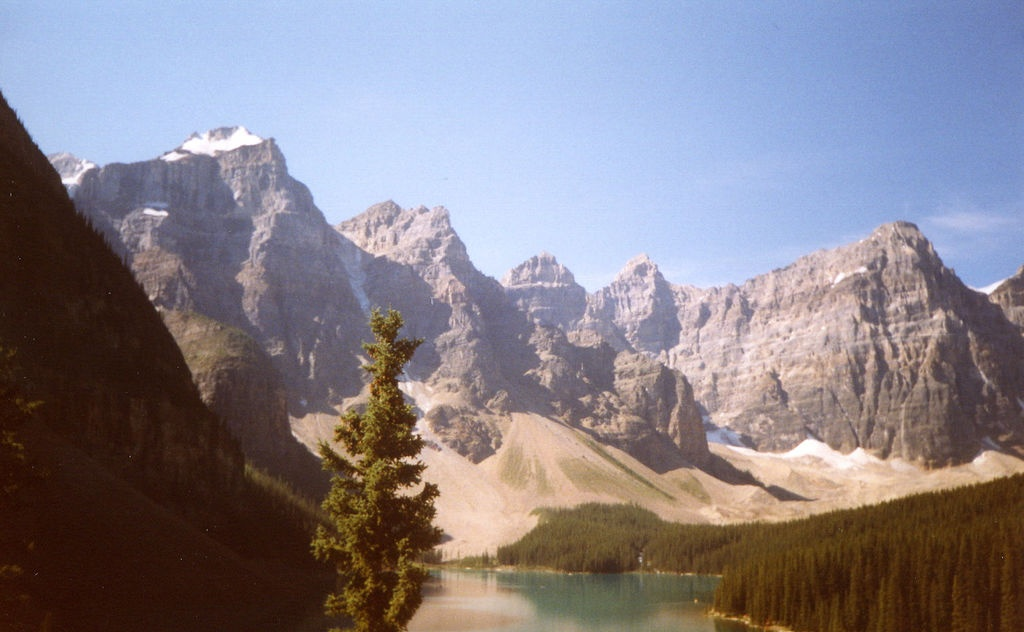
\includegraphics[width = 0.3\textwidth]{images/29018694.jpg}}
\hspace{5mm}
\subfloat{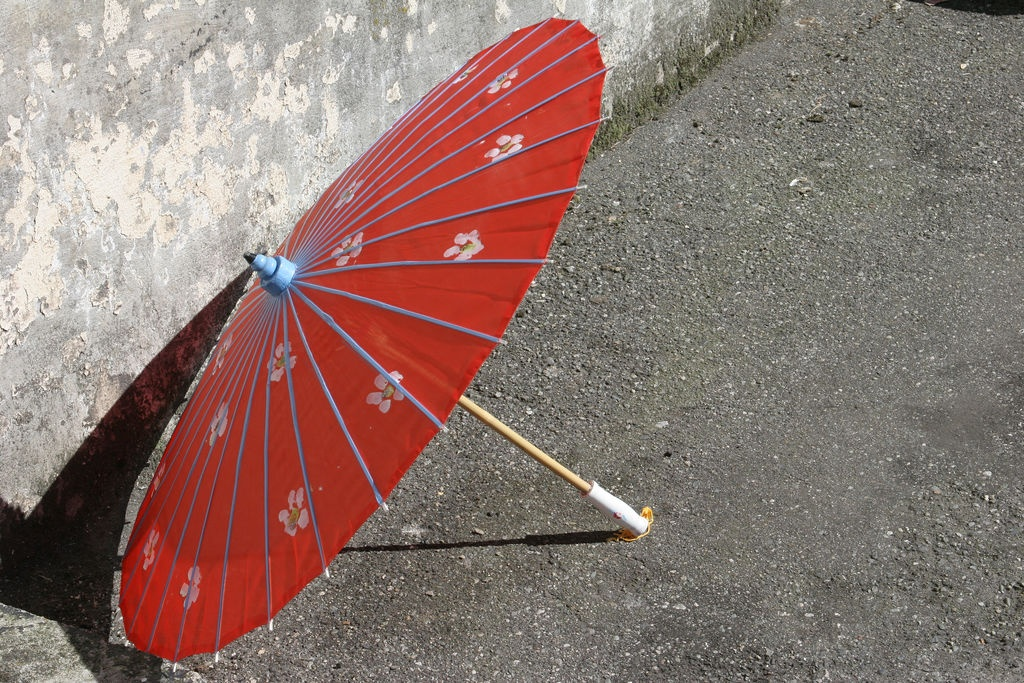
\includegraphics[width = 0.3\textwidth]{images/28874882.jpg}}
\hspace{5mm}
%\subfloat{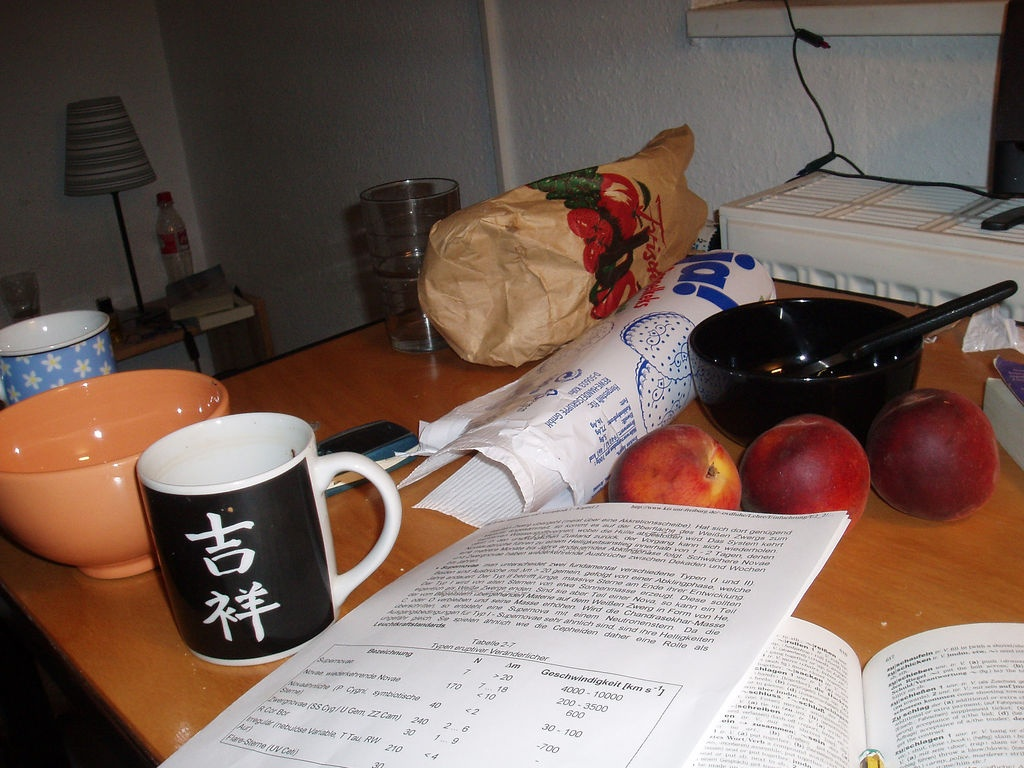
\includegraphics[width = 0.3\textwidth]{images/28848380.jpg}}
%\hspace{5mm}
%\subfloat{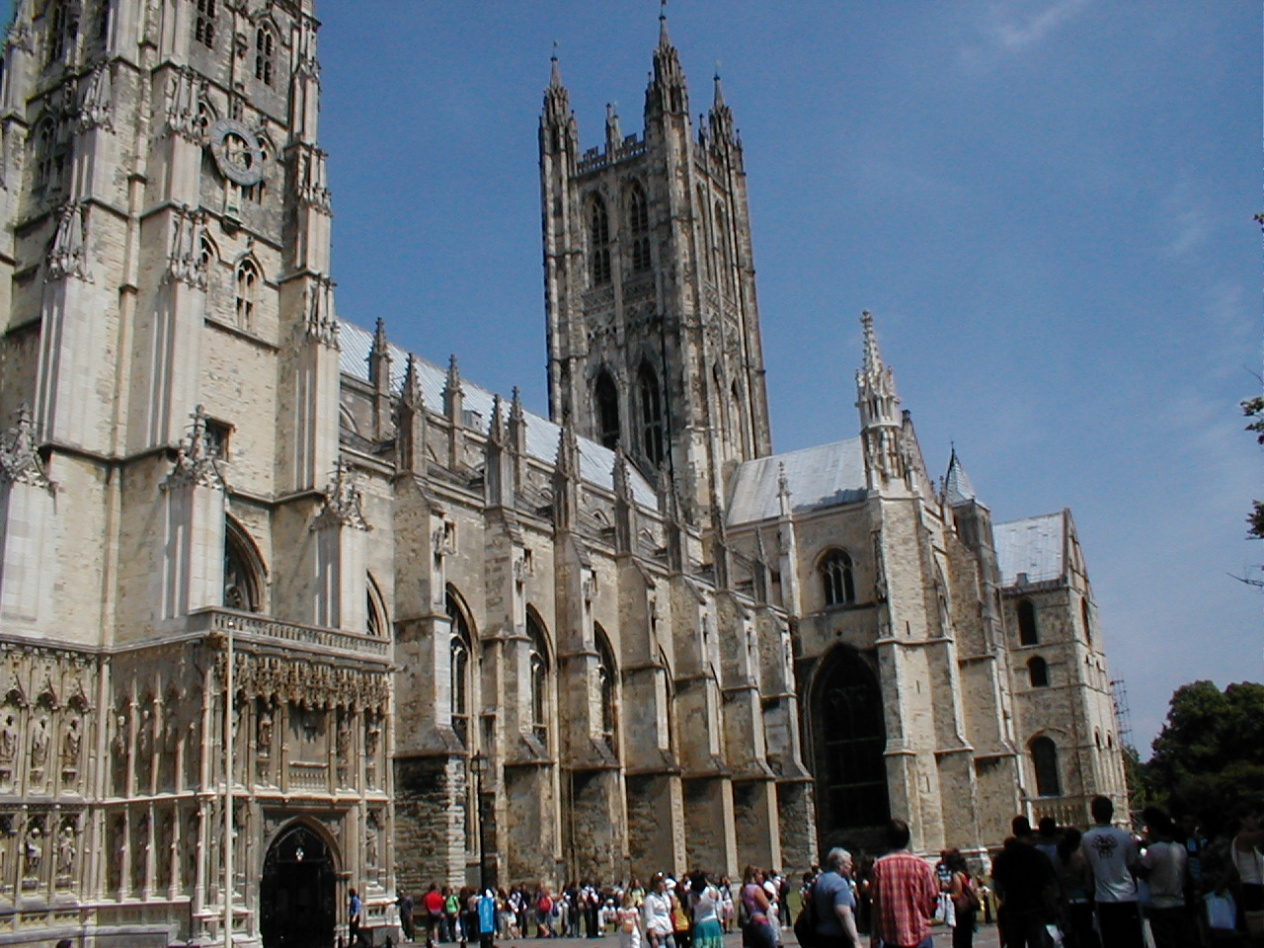
\includegraphics[width = 0.3\textwidth]{images/28859439.jpg}}
%\hspace{5mm}
\subfloat{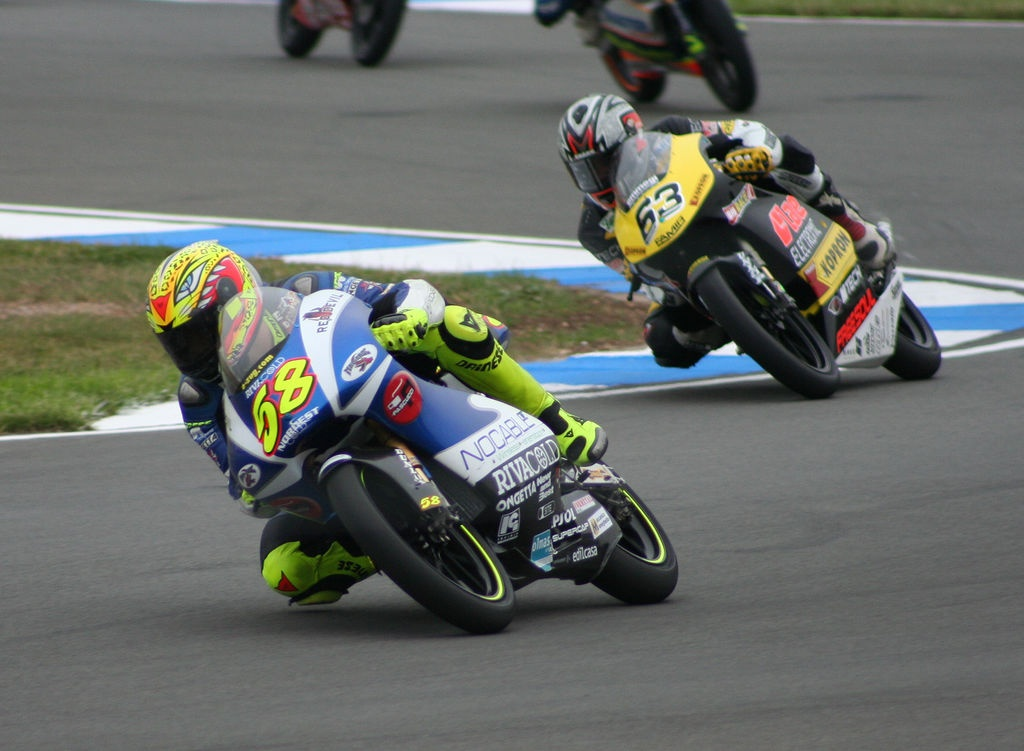
\includegraphics[width = 0.3\textwidth]{images/28803842.jpg}}
\hspace{5mm}
\subfloat{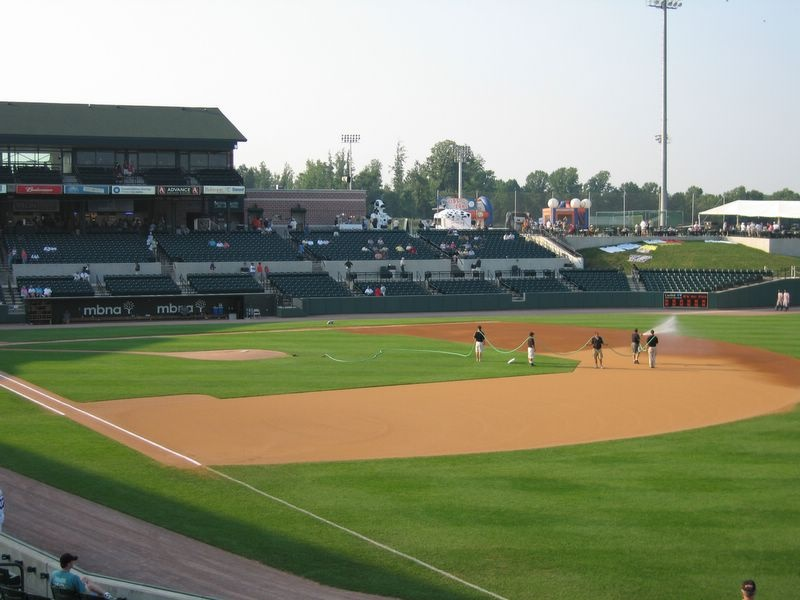
\includegraphics[width = 0.3\textwidth]{images/28894495.jpg}}
\hspace{5mm}
\subfloat{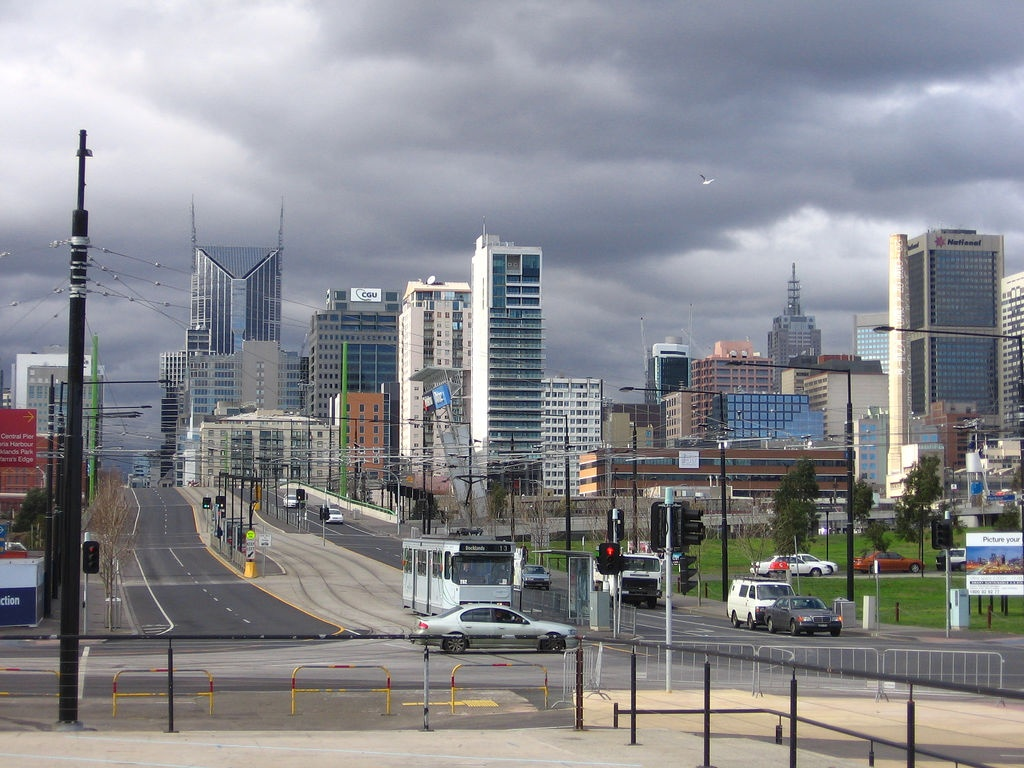
\includegraphics[width = 0.3\textwidth]{images/28952841.jpg}}
\caption{image from training set}
\label{fig:USC-SIPI}
\end{figure}
In addition to this we want to know how good the dictionaries can reconstruct
and compress images outside of the training set. For those comparisons we use a
well known set of standard test images from the \emph{USC-SIPI Image
Database}\footnote{\url{http://sipi.usc.edu/database/}}. They are often
used in image processing for evaluation of compression algorithms. 
Including pictures such as Lena, Mandrill and Peppers.
\begin{figure}[h]
\centering
\subfloat{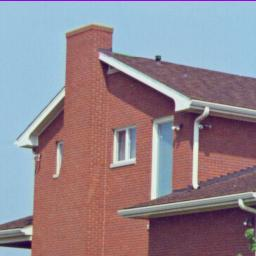
\includegraphics[width = 0.3\textwidth]{images/4_1_05.jpg}}
\hspace{5mm}
\subfloat{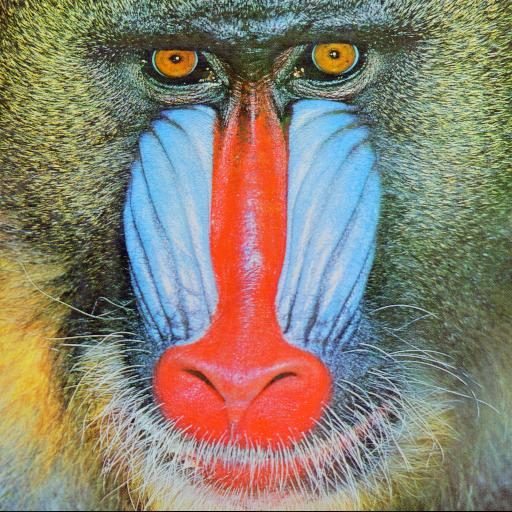
\includegraphics[width = 0.3\textwidth]{images/4_2_03.jpg}}
\hspace{5mm}
\subfloat{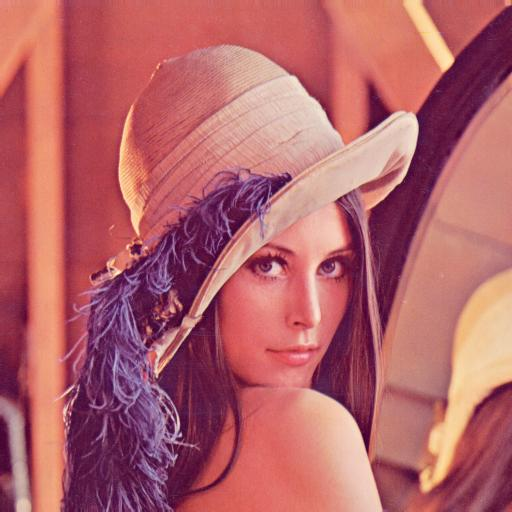
\includegraphics[width = 0.3\textwidth]{images/4_2_04.jpg}}
\hspace{5mm}
\subfloat{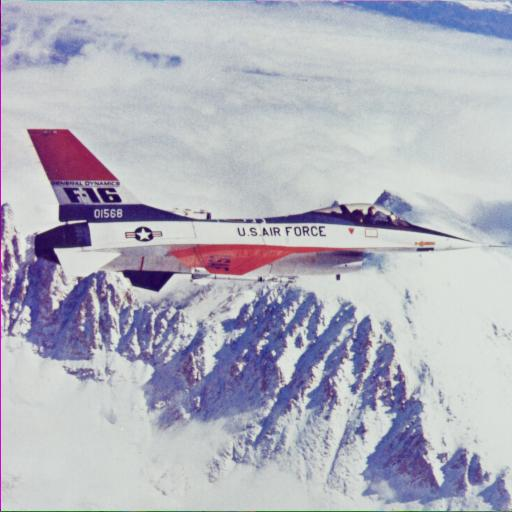
\includegraphics[width = 0.3\textwidth]{images/4_2_05.jpg}}
\hspace{5mm}
\subfloat{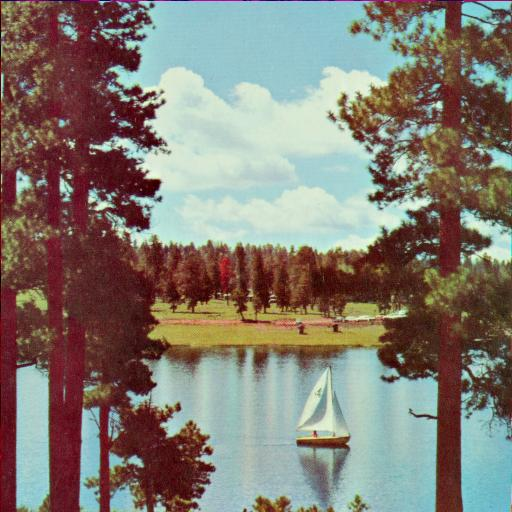
\includegraphics[width = 0.3\textwidth]{images/4_2_06.jpg}}
\hspace{5mm}
\subfloat{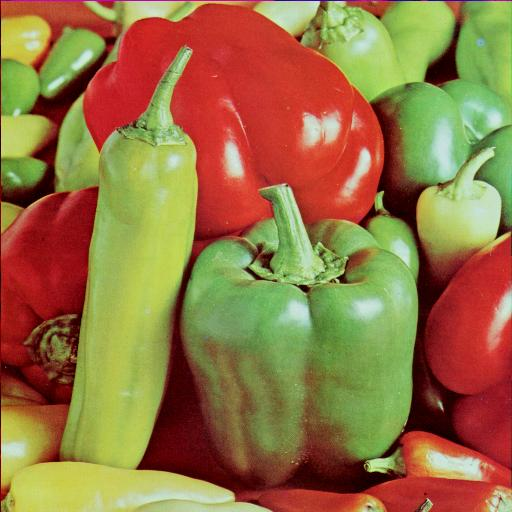
\includegraphics[width = 0.3\textwidth]{images/4_2_07.jpg}}
\caption{images from USC-SIPI Image Database}
\label{fig:USC-SIPI}
\end{figure}

\section{Training sets}
%\subsection{Learning specific dictionaries}
Section \ref{sec:learnForTheTask} mentions that one of the key
elements of the learning algorithms is the learning of specialization
dictionaries. Task specific training data is a common way to solve the problem
of finding  the right dictionary. Here learning for the task comes into
account. Such as de-noising/in-painting dictionaries directly learned from the
initial signal that gets de-noised or restored from in-painting. If the task
gets bigger it sounds logical to increase the size of training data and take a
bigger variety of signals to learn from.  We have a closer look at differences
of learned elements from specific sets of images. These sets include sketches,
still images of animations from Disney and post-impressionistic images from
Vincent van Gogh.  

Are big image collections specific enough to benefit from sparse coding?
%\thispagestyle{empty}

%\section{Experiments}


\chapter{Results}

\section{Single vs. Cluster}
\begin{table}[h]
\caption{single vs. cluster}
\centering
\begin{tabular}{l c c c c c}
\hline\hline
Image & 300 & 600 & 900 & 1800 & 3000 \\
\hline
image 1 & 30 & 30 & 30 & 30 & 30 \\
image 2 & 30 & 30 & 30 & 30 & 30 \\
image 3 & 30 & 30 & 30 & 30 & 30 \\
\hline
\end{tabular}
\end{table}

\begin{figure}
\centering
\subfloat[low pass]{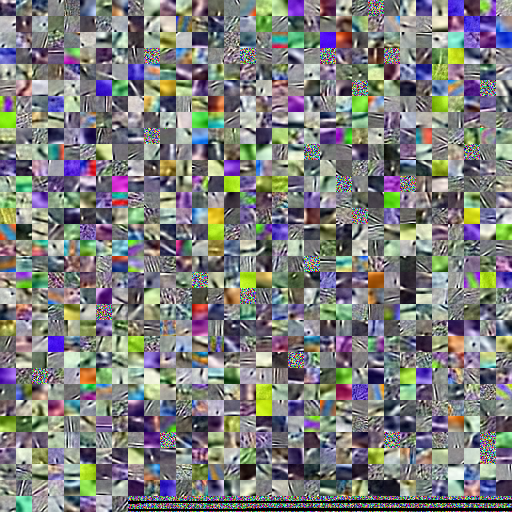
\includegraphics[width =
0.4\textwidth]{images/16_1000_1000_10_lasso.png}}
\hspace{5mm}
\subfloat[high pass]{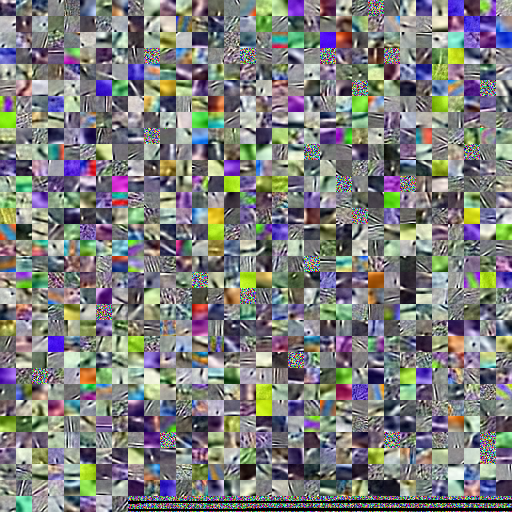
\includegraphics[width =
0.4\textwidth]{images/16_1000_1000_10_lasso.png}}
\caption{low pass}
\label{fig:16_1000_lasso}
\end{figure}
\begin{figure}
\centering
\subfloat[low pass]{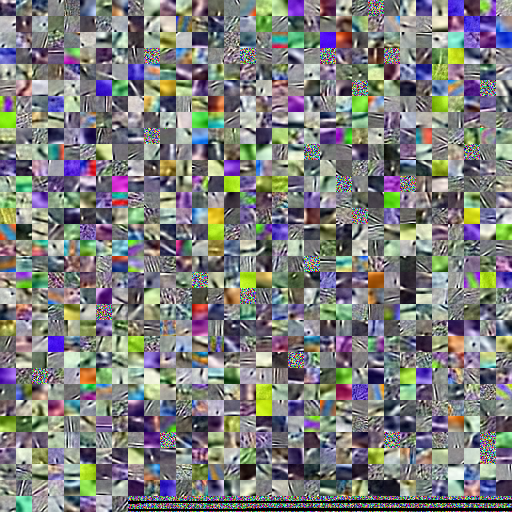
\includegraphics[width =
0.4\textwidth]{images/16_1000_1000_10_lasso.png}}
\hspace{5mm}
\subfloat[high pass]{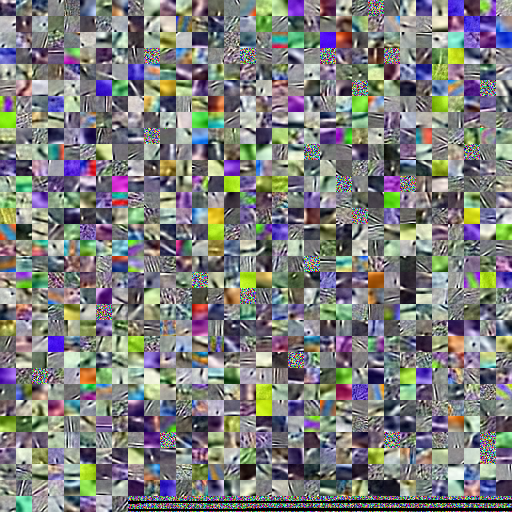
\includegraphics[width =
0.4\textwidth]{images/16_1000_1000_10_lasso.png}}
\caption{low pass}
\label{fig:16_1000_lasso}
\end{figure}
\begin{figure}
\centering
\subfloat[low pass]{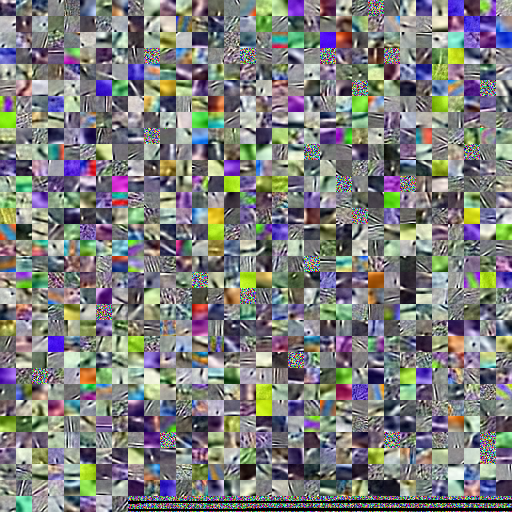
\includegraphics[width =
0.4\textwidth]{images/16_1000_1000_10_lasso.png}}
\hspace{5mm}
\subfloat[high pass]{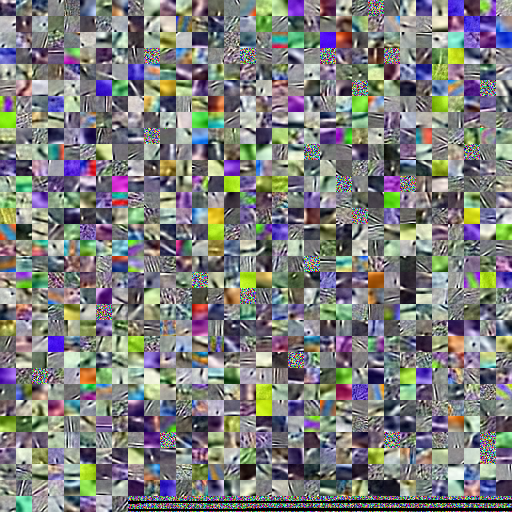
\includegraphics[width =
0.4\textwidth]{images/16_1000_1000_10_lasso.png}}
\caption{low pass}
\label{fig:16_1000_lasso}
\end{figure}

\section{Compression}

\subsection{Natural image database}


\begin{figure}[h]
\centering
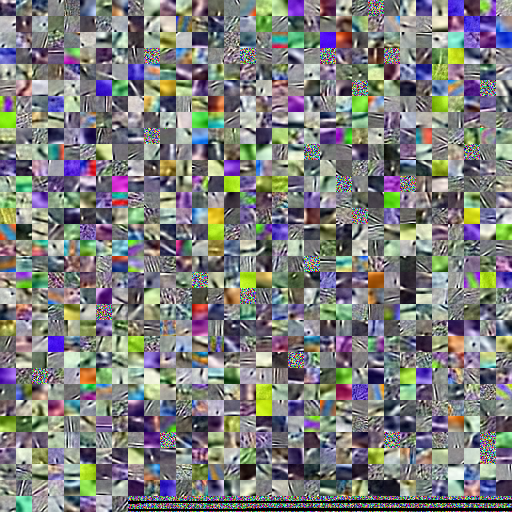
\includegraphics[width = 0.44\textwidth]{images/16_1000_1000_10_lasso.png}
\caption{16x16 LARS-lasso with 1000 elements}
\label{fig:16_1000_lasso}
\end{figure}

\begin{figure}
\centering
\subfloat[low pass]{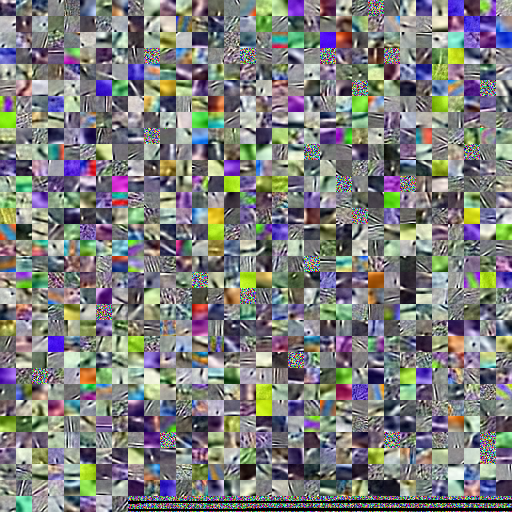
\includegraphics[width =
0.4\textwidth]{images/16_1000_1000_10_lasso.png}}
\hspace{5mm}
\subfloat[high pass]{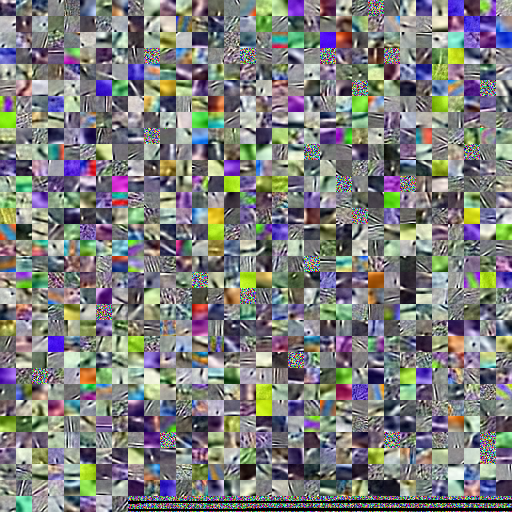
\includegraphics[width =
0.4\textwidth]{images/16_1000_1000_10_lasso.png}}
\caption{low pass}
\label{fig:16_1000_lasso}
\end{figure}
\begin{figure}
\centering
\subfloat[low pass]{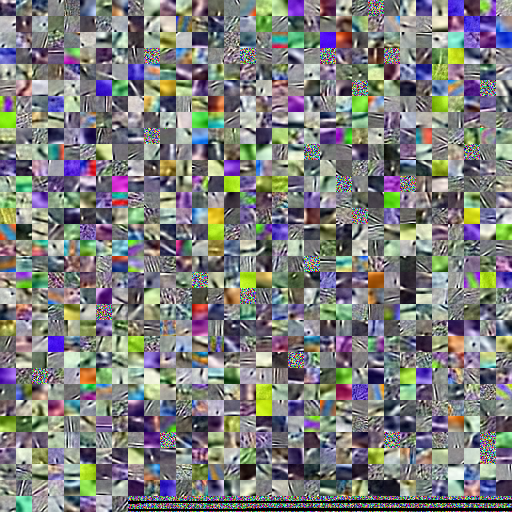
\includegraphics[width =
0.4\textwidth]{images/16_1000_1000_10_lasso.png}}
\hspace{5mm}
\subfloat[high pass]{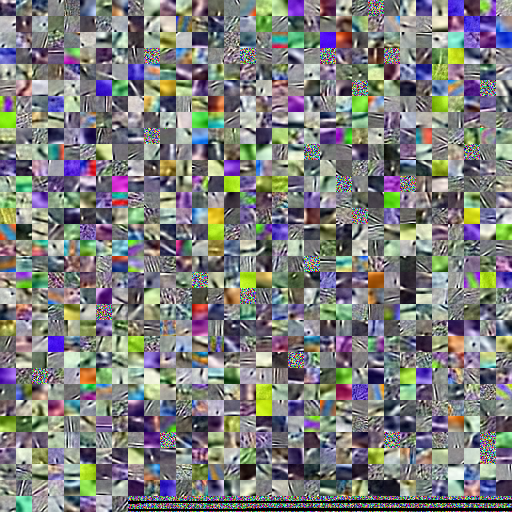
\includegraphics[width =
0.4\textwidth]{images/16_1000_1000_10_lasso.png}}
\caption{low pass}
\label{fig:16_1000_lasso}
\end{figure}
\begin{figure}
\centering
\subfloat[low pass]{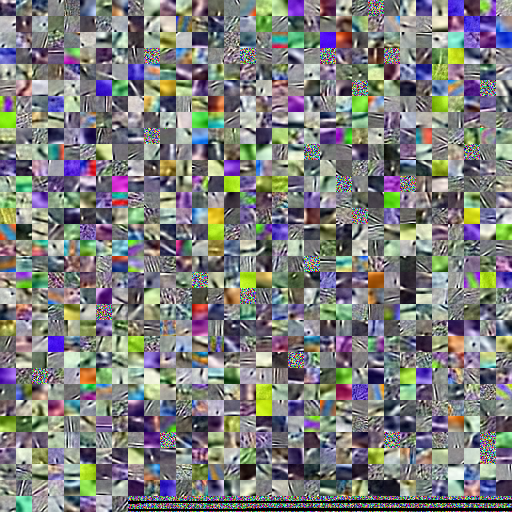
\includegraphics[width =
0.4\textwidth]{images/16_1000_1000_10_lasso.png}}
\hspace{5mm}
\subfloat[high pass]{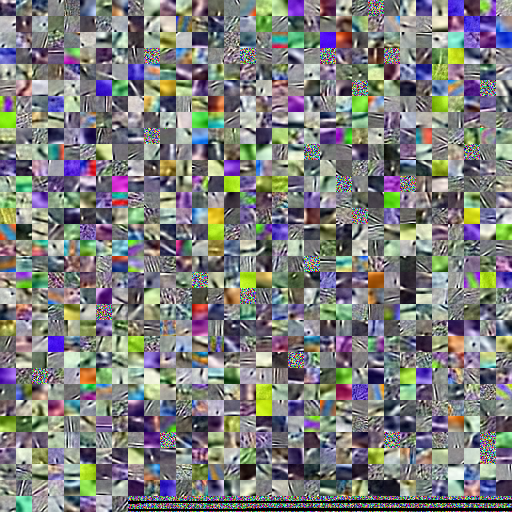
\includegraphics[width =
0.4\textwidth]{images/16_1000_1000_10_lasso.png}}
\caption{low pass}
\label{fig:16_1000_lasso}
\end{figure}



\subsection{Specific image groups}

\begin{figure}[h]
\centering

\includegraphics[width = 0.66\textwidth]{images/1000_sketches.png}
\caption{1000 16x16 elements of sketches database}
\label{fig:16_1000_lasso}
\end{figure}

\begin{figure}
\centering
\subfloat[low pass]{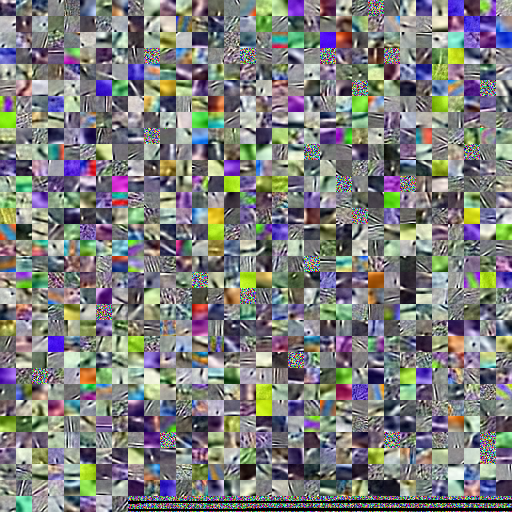
\includegraphics[width =
0.4\textwidth]{images/16_1000_1000_10_lasso.png}}
\hspace{5mm}
\subfloat[high pass]{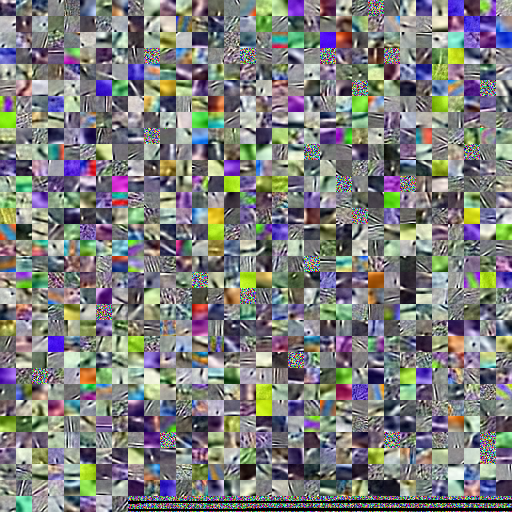
\includegraphics[width =
0.4\textwidth]{images/16_1000_1000_10_lasso.png}}
\caption{low pass}
\label{fig:16_1000_lasso}
\end{figure}
\begin{figure}
\centering
\subfloat[low pass]{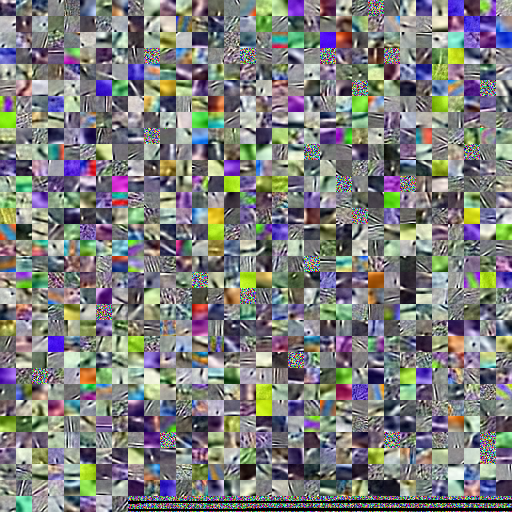
\includegraphics[width =
0.4\textwidth]{images/16_1000_1000_10_lasso.png}}
\hspace{5mm}
\subfloat[high pass]{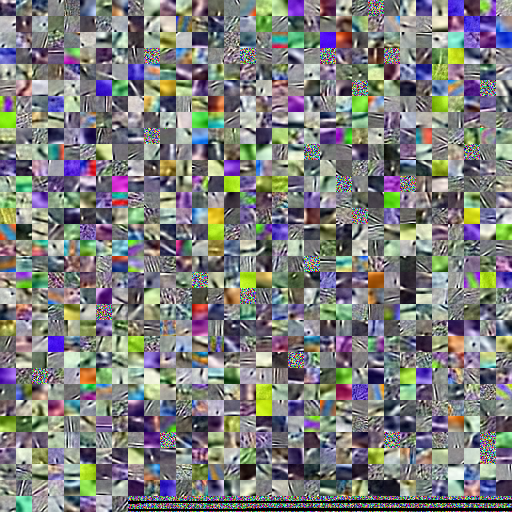
\includegraphics[width =
0.4\textwidth]{images/16_1000_1000_10_lasso.png}}
\caption{low pass}
\label{fig:16_1000_lasso}
\end{figure}
\begin{figure}
\centering
\subfloat[low pass]{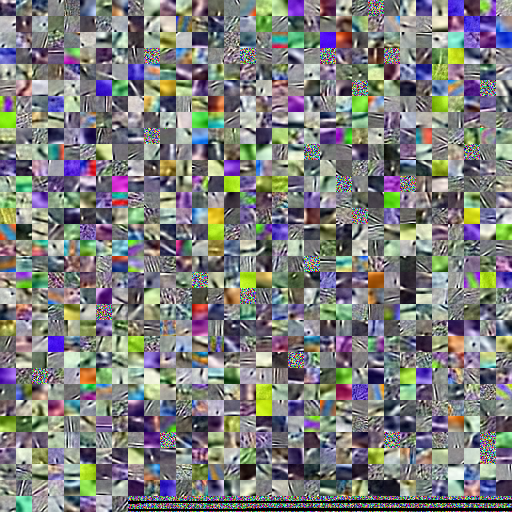
\includegraphics[width =
0.4\textwidth]{images/16_1000_1000_10_lasso.png}}
\hspace{5mm}
\subfloat[high pass]{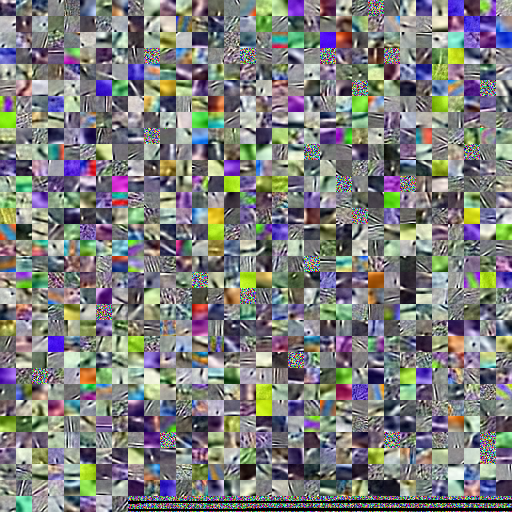
\includegraphics[width =
0.4\textwidth]{images/16_1000_1000_10_lasso.png}}
\caption{low pass}
\label{fig:16_1000_lasso}
\end{figure}
%\section{Quality}
%\subsection*{trained vs. analytical base}
%\subsection*{Compression ratio}
%\subsection*{Dictionary size}
%Setup:
%  initialize: random pixels, radom samples 
%  dict size: 256, 1000, 4000, 8000
%  coeffs: 5, 10, 20









